\section{Method}

CoEvoP\&R searches the differentiable placement objective while keeping
DREAMPlace's optimizer fixed. This isolates objective quality and permits new
interactions among wirelength, density, routing pressure, and timing-relevant
observables that fixed-form parameter tuning cannot express.
Figure~\ref{fig:loop} shows the loop: archive-conditioned proposal, restricted
lowering, cost-scaled EDA evaluation, and feedback reconstruction. The LLM
neither invokes the EDA tools nor selects fitness.

\subsection{Problem Formulation}
\label{sec:problem}

Let $d\in\mathcal{D}$ denote a design, $s$ a placement seed, and
$\mathbf{x}$ the positions of all movable macros and standard cells. A
candidate objective $f$ produces the mixed-size placement
\begin{equation}
\mathbf{x}_{d,s}(f)=\mathcal{P}_{d,s}(f),
\label{eq:placement-map}
\end{equation}
where $\mathcal{P}_{d,s}$ is DREAMPlace with its native objective replaced by
$f$; the optimizer and downstream evaluators remain fixed.

Let $\mathcal{T}=\{t_1,\ldots,t_k\}$ contain the allowed differentiable
observables. The first call records each term scale $\kappa_j$, which remains
fixed for the run. A complete replacement objective is
\begin{equation}
\widetilde t_j(\mathbf{x};d)=
\frac{t_j(\mathbf{x};d)}{\kappa_j},\qquad
f_\theta(\mathbf{x};d)=\kappa_{\mathrm{wl}}
F_\theta\!\left(\widetilde{\mathcal{T}}(\mathbf{x};d)\right),
\label{eq:candidate-objective}
\end{equation}
where restricted program $F_\theta$ has one wirelength and one density anchor;
routing terms and nonlinear interactions are optional.
$\kappa_{\mathrm{wl}}$ restores wirelength scale. The expression, constants,
term set, and named diagnostics form its lowered \texttt{ObjectiveSpec}.
Equation~\eqref{eq:candidate-objective} defines the entire minimized objective,
not a residual around a hidden native loss.

For evaluator $E_j$, define
$m_j(f;d,s)=E_j(\mathbf{x}_{d,s}(f))$ and let $f_0$ denote native
DREAMPlace. CoEvoP\&R orients every metric so that positive gain is better:
\begin{equation}
g_j(f;d,s)=o_j\,
\frac{m_j(f;d,s)-m_j(f_0;d,s)}{\nu_j},
\quad o_j\in\{-1,+1\},
\label{eq:metric-gain}
\end{equation}
where $o_j=-1$ for costs, $o_j=+1$ for WNS and TNS, and $\nu_j>0$ is a
fixed panel-specific scale. Density overflow measures placement feasibility;
routing congestion and routed wirelength come only from the routed evaluator.

Search-panel evidence guides parent selection; final-panel metrics never enter
prompts or archive fitness. Budgets $B_A,B_B,B_C$ bound placement, timing, and
routing calls. Selection of the returned objective is restricted to candidates
with Tier-C evidence:
\begin{equation}
f^*=\arg\max_{f\in\mathcal{A}^{C}_G}S_{\mathrm{final}}(f),
\quad N_\ell\leq B_\ell,\ \ell\in\{A,B,C\},
\label{eq:routed-objective}
\end{equation}
where $\mathcal{A}^{C}_G$ is the routed subset of the final archive. Thus,
search guidance and final evidence remain disjoint.

\subsection{Archive-Conditioned Proposal}
\label{sec:proposer}

Evolution starts from a measured portfolio of native-equivalent, alternative
wirelength-density, density-heavy, and routing-aware formulas. Valid symbolic
seeds populate the islands of $\mathcal{A}_0$; native DREAMPlace remains an
external, uneditable reference. Each island receives a measured eligible seed
before LLM sampling.

The controller rotates across islands and samples a parent from the current
island's eligible MAP-Elites cells. Let $S_A(p)$ be the constrained Tier-A
score defined below, $d_{\mathrm{base}}(p)\in[0,1]$ the distance from the
nearest fixed mechanism, and $n_g(\mathrm{sig}(p))$ the number of candidates
with the same mechanism signature. The implemented novelty-aware distribution
is
\begin{equation}
\begin{aligned}
\pi_{\mathrm{par}}(p\mid\mathcal{A}_g)
&=\frac{w_g(p)}{\sum_{u\in\mathcal{P}_g}w_g(u)},\\
w_g(p)&=\max\{\log(1+[S_A(p)]_+),\epsilon\}\\
&\quad\times\frac{\tfrac12+d_{\mathrm{base}}(p)}
{\sqrt{n_g(\mathrm{sig}(p))}}.
\end{aligned}
\label{eq:parent-policy}
\end{equation}
for $p$ in parent pool $\mathcal{P}_g$, which contains admitted elites and
bounded, behaviorally distinct near misses but excludes structural failures
and severe regressions. The mechanism-count denominator prevents repeated
sampling of one family.

The prompt never contains the full archive. Retrieval constructs
\begin{equation}
\begin{aligned}
\mathcal{H}_g={}&\{f_0,p_g\}\cup\operatorname{Top}(\mathcal{A}_g)
\cup\operatorname{Diverse}(\mathcal{A}_g,\phi)\\
&\cup\operatorname{NearMiss}(\mathcal{A}_g)
\cup\operatorname{RelevantFail}(\mathcal{A}_g,p_g).
\end{aligned}
\label{eq:retrieval-policy}
\end{equation}
The bounded sets provide a champion, high scorers, behaviorally diverse cells,
useful tradeoffs, and failures relevant to the selected parent's terms.
Duplicate programs are removed unless measured outcomes differ. The controller
then builds
\begin{equation}
\Pi_g=\bigl(\underbrace{r,\iota,b,\sigma}_{\text{fixed contract}},
\underbrace{p_g,u_g,\mathbf{m}_g,\mathcal{H}_g}_{\text{measured context}}\bigr),
\label{eq:prompt-packet}
\end{equation}
where $(r,\iota,b,\sigma)$ fixes the task, objective API, target context, and
JSON schema. Adaptive fields supply the parent, edit mode, evaluator scorecard,
and retrieved programs. Gate thresholds remain hidden so that proposals use
measured behavior rather than copy admission rules.

The controller normally requests a SEARCH/REPLACE edit and switches to a full
rewrite after repeated static rejection. A stateless provider produces $K$
independent responses from the same packet:
\begin{equation}
\mathcal{S}_g=\left\{L_{\mathcal{G}}(y_{g,i})\mid
y_{g,i}\sim q_\lambda(\cdot\mid\Pi_g),\;
L_{\mathcal{G}}(y_{g,i})\neq\bot\right\}_{i=1}^{K}.
\label{eq:candidate-set}
\end{equation}
Each response contains \texttt{id}, \texttt{rationale},
\texttt{parent\_ids},
\texttt{declared\_\allowbreak term\_\allowbreak usage},
\texttt{change\_\allowbreak description}, and a complete
\texttt{objective\_\allowbreak program}. Provider retries repair malformed or rejected
responses within the same sample. Deterministic coefficient siblings calibrate
accepted routing mechanisms; they share one lineage, but each consumes
evaluator budget.

Figure~\ref{fig:prompt-schema} exposes the proposal and lowering contracts.
It also distinguishes independent samples from retries and generated code from
the executable record.

\begin{figure}[t]
\centering
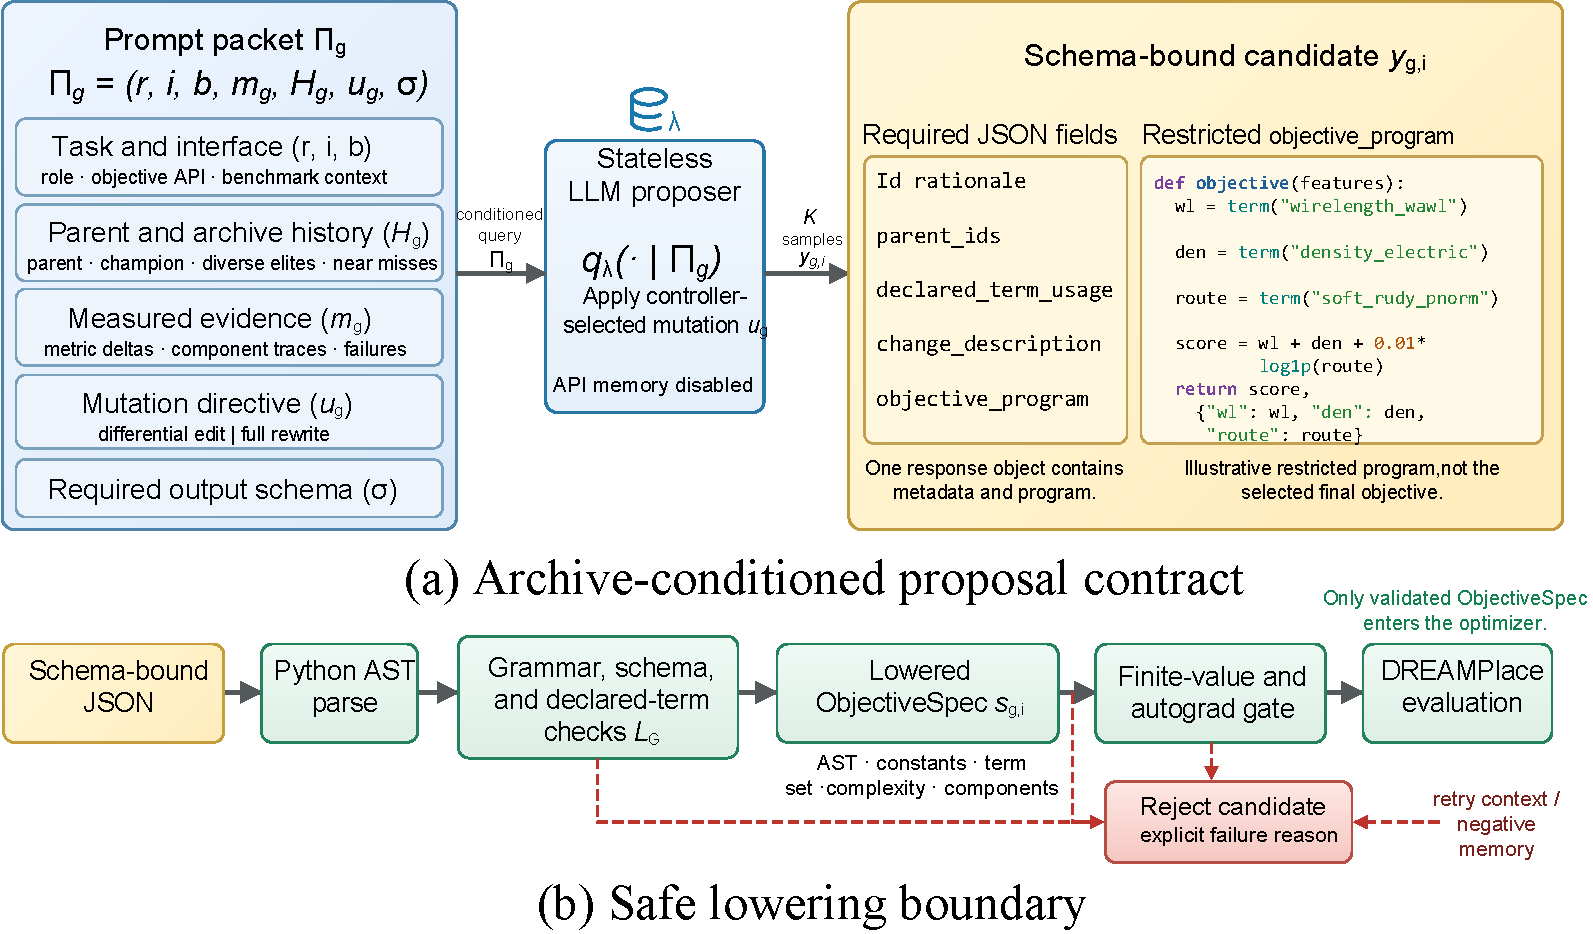
\includegraphics[width=\columnwidth]{graphs/Figure2.pdf}
\caption{Proposal and lowering contracts. (a) A fixed objective interface and
measured archive context condition $K$ stateless LLM samples. (b) Schema, AST,
term, and autograd checks lower a valid response into \texttt{ObjectiveSpec};
rejections return an explicit retry or negative-memory record.}
\Description{An archive-conditioned prompt supplies task, parent, measured
evidence, mutation, and schema context to a stateless LLM. A schema-bound
candidate is parsed and lowered into an ObjectiveSpec. Static or autograd
failures produce explicit rejection feedback, and only valid records reach
DREAMPlace.}
\label{fig:prompt-schema}
\end{figure}

\subsection{Safe Objective Lowering}
\label{sec:safe-interface}

The lowering boundary makes the model's action space finite. Static admission
validates JSON, parses the Python AST as data, checks declared against observed
terms, and lowers score and component expressions into \texttt{ObjectiveSpec}:
\begin{equation}
L_{\mathcal{G}}(y)=
\begin{cases}
s, & \mathrm{static}_{\mathcal{G}}(y)=1,\\
\bot, & \text{otherwise}.
\end{cases}
\label{eq:lowering-map}
\end{equation}
The grammar permits constants, local assignments, named \texttt{term} calls,
arithmetic, safe division, and \texttt{log1p}, \texttt{sqrt}, \texttt{square},
\texttt{softplus}, and \texttt{sigmoid}. It rejects control flow, imports,
arbitrary calls, mutation, randomness, and direct feature access. AST depth is
at most five, with 12 primitives per expression and six returned diagnostics.

Terms include weighted-average and log-sum-exp wirelength; electric and
bell-shaped density; soft-RUDY mean and hotspot pressure; and long-net,
pin-density, and pin-count-weighted pressure. Static compatibility requires
exactly one wirelength and one density family and rejects unavailable terms,
baseline clones, and out-of-range routing coefficients. Nonlinear interactions
remain expressible without duplicated anchors or ill-scaled objectives.

Dynamic admission occurs on the first DREAMPlace objective call. DREAMPlace
evaluates only the lowered AST, differentiates the resulting scalar, and
allows optimization to continue only when
\begin{equation}
\begin{aligned}
\mathcal{F}_{\mathrm{safe}}=\{f_s\mid{}&
\mathrm{terms}(f_s)\subseteq\mathcal{T},\quad
|f_s(\mathbf{x}_0)|<\infty,\\
&0<\|\nabla_{\mathbf{x}}f_s(\mathbf{x}_0)\|_2<\infty,\quad
\mathrm{compat}(f_s)=1\}.
\end{aligned}
\label{eq:safe-family}
\end{equation}
Runtime guards repeat finite checks throughout placement and terminate at the
first invalid state. The initial autograd gate establishes local executability;
the guards catch later instability. Raw model code is never imported or
executed.

\subsection{Cost-Scaled Evaluation}
\label{sec:cascade}
\label{sec:proxy-audit}

Expensive evidence is allocated only after optimizer compatibility. Tier~A
runs each admitted objective on a multi-design DREAMPlace panel and records
HPWL, density overflow, runtime, convergence, gradient behavior, per-design
outcomes, and component trajectories. Tier~B adds placement-RC timing when
collateral exists: search uses FLUTE/Elmore, while final WNS/TNS use OpenTimer
and are not called post-route timing. Tier~C routes scheduled promotions
through OpenROAD/ChiPBench and records global-route wirelength, routed
congestion or overflow, available post-GRT timing, runtime, and failure stage.

Tier~A first applies feasibility and robustness constraints. Let
$\bar g_H,\bar g_D$ denote mean HPWL and density-overflow gains,
$g_H^{\min},g_D^{\min}$ their worst-design gains, and $q_{HD}$ the fraction of
designs improving both metrics. The admission indicator is
\begin{equation}
\begin{aligned}
\chi_A(f)=\mathbb{I}\bigl[{}&
\bar g_H\geq-\delta_H,\quad \bar g_D\geq0,\\
&g_H^{\min}\geq-\delta_H^d,\quad
g_D^{\min}\geq-\delta_D^d,\\
&n_{\mathrm{struct}}=n_{\mathrm{severe}}=0\bigr],
\end{aligned}
\label{eq:parent-gate}
\end{equation}
where fixed tolerances admit bounded HPWL and per-design numerical noise. The
search score is
\begin{equation}
\begin{aligned}
S_A(f)=\chi_A(f)\biggl(&w_H[\bar g_H]_+ +w_D[\bar g_D]_+
+\frac{w_R}{1+\bar r_A(f)}\\
&+w_Qq_{HD}(f)-\eta c(f)\biggr),
\end{aligned}
\label{eq:selection-score}
\end{equation}
where $[z]_+=\max(z,0)$, $\bar r_A$ averages rank across design-seed cells, and
$c(f)$ is complexity. Weights and tolerances are fixed before a run. An elite
must also beat the same-flow fixed-objective portfolio and Pareto-improve over
its strongest HPWL/overflow member. Bounded distinct tradeoffs may enter
$\mathcal{P}_g$ as near misses but cannot become routed finalists before
passing the elite gate.

Cheap timing signals affect selection only when they add information beyond
HPWL. For timing delta $q\in\{\Delta\mathrm{WNS},\Delta\mathrm{TNS}\}$, the
perturbation audit computes
\begin{equation}
\rho_H(q)=\max\left\{
|\mathrm{Pearson}(\Delta\mathrm{HPWL},q)|,
|\mathrm{Spearman}(\Delta\mathrm{HPWL},q)|\right\}.
\label{eq:proxy-correlation}
\end{equation}
Let $a_C(q)$ indicate that held-out routed promotions preserve the proxy's rank
direction for the corresponding downstream timing metric. Its selection weight
is
\begin{equation}
\gamma_q=a_C(q)
\begin{cases}
0, & \rho_H(q)>0.95,\\
\gamma_{\mathrm{tie}}, & 0.70\leq\rho_H(q)\leq0.95,\\
\gamma_{\mathrm{soft}}, & \rho_H(q)<0.70,
\end{cases}
\quad 0<\gamma_{\mathrm{tie}}<\gamma_{\mathrm{soft}}\leq1.
\label{eq:proxy-admission}
\end{equation}
Until enough routed samples exist, $a_C(q)=0$ and timing remains diagnostic.
Low HPWL correlation establishes non-redundancy; routed agreement establishes
downstream relevance.

Every $\tau_C$ generations, at most $k_C$ unrouted elites are promoted while
$N_C<B_C$. The batch mixes high-$S_A$ candidates with strong occupants of
uncovered mechanism cells, then removes duplicate ASTs and signatures. Tier-C
results are committed before $\Pi_{g+1}$. The final score compares only
candidates with matched downstream evidence:
\begin{equation}
S_{\mathrm{final}}(f)=
\frac{1}{1+\bar r_C(f)}-\eta_Cc(f),
\label{eq:final-score}
\end{equation}
where $\bar r_C$ averages rank over reported post-GRT metrics and $\eta_Cc(f)$
favors compact objectives only when ranks tie.

\subsection{Archive and Closed-Loop Feedback}
\label{sec:archive}
\label{sec:search}

Each archive record contains parent, island, generation, prompt, provider
snapshot and decoding settings, raw response, lowered AST, terms, components,
complexity, tool configuration, per-design metrics, trajectories, artifacts,
and failure reason. Structural failures and completed regressions remain
queryable as negative memory but cannot occupy elite cells; near misses are
exploration-only.

MAP-Elites assigns each parent-eligible candidate to
\begin{equation}
\phi(f)=\bigl(b_{\mathrm{size}}(f),m(f),b_{\mathrm{hpwl}}(f),
b_{\mathrm{dens}}(f),b_{\mathrm{timing}}(f)\bigr),
\label{eq:archive-key}
\end{equation}
where $m(f)$ identifies wirelength-density, route-pressure, long-net,
pin-pressure, fanout-weighted, or hybrid mechanisms; missing timing maps to an
unknown bucket. Each island retains the strongest eligible program per cell:
\begin{equation}
\mathcal{A}_{g+1}[b]=
\arg\max_{u\in\mathcal{A}_g[b]\cup\{f\}}S_A(u),
\qquad b=\phi(f).
\label{eq:archive-update}
\end{equation}
Ring migration periodically copies eligible cell elites into neighboring
islands, where the same cell-replacement rule applies.

Feedback reconstruction converts tool records into compact, actionable
evidence:
\begin{equation}
\begin{aligned}
\mathbf{m}_{g+1}=\operatorname{Summarize}\bigl(&
\Delta\mathrm{rank},\Delta\mathrm{metric},
\mathbf{z}_{\mathrm{design}},\\
&\mathbf{z}_{\mathrm{comp}},\mathbf{z}_{\mathrm{fail}},
\mathbf{z}_{\mathrm{route}}\bigr).
\end{aligned}
\label{eq:feedback-summary}
\end{equation}
$\mathbf{z}_{\mathrm{design}}$ reports per-design and worst-case behavior.
$\mathbf{z}_{\mathrm{comp}}$ stores each component's start/mid/end, range,
mean, trend, and saturation status. $\mathbf{z}_{\mathrm{fail}}$ records
parser, gradient, convergence, and flow failures with repair lessons.
$\mathbf{z}_{\mathrm{route}}$ identifies which placement gains survive routing.
Equation~\eqref{eq:retrieval-policy} selects the programs that accompany this
scorecard in the next prompt.

CoEvoP\&R couples objective evolution to progressively updated placement and
routing evidence without training or mutating the EDA tools. Each routed
promotion can change parent selection, retrieval, or failure context.
Checkpointed prompts, responses, lowered records, metrics, and artifacts make
lineages auditable despite nondeterministic providers. Algorithm~\ref{alg:objective-evolution}
summarizes the loop.

\begin{algorithm}[t]
\caption{CoEvoP\&R objective evolution}
\label{alg:objective-evolution}
\scriptsize
\begin{algorithmic}[1]
\REQUIRE $\mathcal{G},\mathcal{D}_S,\mathcal{B}$;
$G,K,B_A,B_B,B_C,\tau_C,k_C,\tau_{\mathrm{mig}}$
\ENSURE Archive $\mathcal{A}_G$ and routed objective $f^*$
\STATE $\mathcal{A}_0\leftarrow\mathrm{EvaluateSeeds}(\mathcal{B},\mathcal{D}_S)$;
$N_A,N_B,N_C\leftarrow0$
\FOR{$g=0,\ldots,G-1$}
  \STATE $i\leftarrow g\bmod I$;
  $p_g\sim\pi_{\mathrm{par}}(\cdot\mid\mathcal{A}_g^{(i)})$
  \STATE $\mathcal{H}_g\leftarrow\mathrm{Retrieve}(\mathcal{A}_g,p_g)$;
  $u_g\leftarrow\mathrm{DiffOrRewrite}(\mathcal{A}_g,p_g)$
  \STATE $\Pi_g\leftarrow\mathrm{Prompt}(p_g,u_g,\mathbf{m}_g,\mathcal{H}_g)$;
  $\mathcal{Y}_g\leftarrow\{y_{g,j}\}_{j=1}^{K}\sim q_\lambda(\cdot\mid\Pi_g)$
  \FOR{$y\in\mathcal{Y}_g$}
    \STATE $s\leftarrow L_{\mathcal{G}}(y)$
    \IF{$s=\bot$}
      \STATE $\mathrm{RememberFailure}(y)$; \textbf{continue}
    \ENDIF
    \FOR{$f\in\mathrm{Calibrate}(s)$}
      \IF{$N_A\geq B_A$} \STATE \textbf{break} \ENDIF
      \STATE $\mathbf{m}_A\leftarrow E_A(f,\mathcal{D}_S)$; $N_A\leftarrow N_A+1$
      \STATE $\mathbf{m}_B\leftarrow\varnothing$; run $E_B(f)$ and increment $N_B$
      only if proxy-admitted and $N_B<B_B$
      \STATE $\mathcal{A}_g\leftarrow\mathrm{Insert}(\mathcal{A}_g,f,\mathbf{m}_A,\mathbf{m}_B)$
    \ENDFOR
  \ENDFOR
  \IF{$(g+1)\bmod\tau_C=0$ and $N_C<B_C$}
    \STATE $\mathcal{C}_g\leftarrow\mathrm{Promote}(\mathcal{A}_g,k_C,B_C-N_C)$
    \STATE $\mathbf{m}_C\leftarrow E_C(\mathcal{C}_g)$;
    $N_C\leftarrow N_C+|\mathcal{C}_g|$
    \STATE $\mathrm{CommitRoutedFeedback}(\mathcal{A}_g,\mathbf{m}_C)$
  \ENDIF
  \STATE $\mathcal{A}_{g+1}\leftarrow\mathrm{Migrate}(\mathcal{A}_g)$ if scheduled,
  else $\mathcal{A}_g$
\ENDFOR
\STATE \RETURN $\mathcal{A}_G,
f^*=\arg\max_{f\in\mathcal{A}^{C}_G}S_{\mathrm{final}}(f)$
\end{algorithmic}
\end{algorithm}
